\documentclass[10pt]{article}
\usepackage{geometry}
\geometry{a4paper, portrait, margin=1in}
% \author{Lawrence Liu}
\usepackage{subcaption}
\usepackage{graphicx}
\usepackage{float}
\usepackage{amsmath}
\usepackage{pdfpages}
\newcommand{\Laplace}{\mathscr{L}}
\DeclareMathOperator{\Tr}{tr}
\setlength{\parskip}{\baselineskip}%
\setlength{\parindent}{0pt}%
\usepackage{xcolor}
\usepackage{listings}
\definecolor{backcolour}{rgb}{0.95,0.95,0.92}
\usepackage{amssymb}
\lstdefinestyle{mystyle}{
    backgroundcolor=\color{backcolour}}
\lstset{style=mystyle}

\title{A Kernel Density Based Approach to Portfolio Optimization}
\author{Lawrence Liu}
\date{June 2023}
% \begin{abstract}
%     TODO
% \end{abstract}
\begin{document}
\maketitle
\begin{abstract}
    In this paper we propose a new approach to portfolio optimization. 
    We show that the returns of the assets are not normally distributed, and thus we develop a new approach 
    that does not rely on this assumption, unlike Modern Portfolio Theory. We show that this method 
    provides a higher Sharpe Ratio and a higher Year over Year return compared to Modern Portfolio Theory.
\end{abstract}
\section{Introduction}
Portfolio optimization can be characterized as a constrained optimization problem, where we want to maximize the expected return 
of a portfolio while minimizing the risk. The risk is usually measured by the standard deviation of the portfolio. If we allow margin trading,
meaning that we can borrow money to invest, and thus have a position larger than our initial capital, then the optimal 
portfolio becomes a scaling of the portfolio that maximizes the Sharpe ratio, this is what we call the efficient frontier. We define the 
sharpe ratio as the ratio of the expected return of the portfolio to the standard deviation of the portfolio.
\begin{equation}
    \text{Sharpe Ratio} = \frac{\mu_p}{\sigma_p}
\end{equation}
Where $\mu_p$ is the expected return of the portfolio, and $\sigma_p$ is the standard deviation of the portfolio. If we take the $\mu_p$
as the average day to day return of the portfolio, and $\sigma_p$ as the standard deviation of the day to day returns, then we can 
also define the annualized Sharpe ratio as
\begin{equation}
    \text{Sharpe Ratio} = \frac{\mu_p}{\sigma_p}\sqrt{252}
\end{equation}
Where 252 is the number of trading days in a year. From now on we use the annualized Sharpe ratio and all further references 
to Sharpe ratio will be the annualized Sharpe ratio.
\subsection{Modern Portfolio Theory}
The most common approach to create the portfolio that maximizes the Sharpe ratio is Modern Portfolio Theory (MPT). MPT was first
introduced by Harry Markowitz in 1952 \cite{markowitz1952portfolio}. Let us define
the sample mean of the returns of the assets as $\mu$, and the sample covariance matrix of the returns of the assets as $\Sigma$. Then $\mu_p$
and $\sigma_p$ can be written as
\begin{equation}
    \mu_p = w^T\mu
\end{equation}
\begin{equation}
    \sigma_p = \sqrt{w^T\Sigma w}
\end{equation}
Where $w$ is the weight vector of the portfolio. The optimization problem can then be written as
\begin{equation}
    \begin{aligned}
        & \underset{w}{\text{maximize}}
        & & \frac{w^T\mu}{\sqrt{w^T\Sigma w}} \\
        & \text{subject to}
        & & \sum_{i=1}^n w_i = 1 \\
        & & & w_i \geq 0 \quad \forall i \in \{1, \dots, n\}
    \end{aligned}
\end{equation}
Where $n$ is the number of assets in the portfolio. This is a fractional programming problem which we can solve in the following manner.\cite{its_convex_if_you_tilt_your_head_a_bit} 
If we let $y=\alpha w$, where $\alpha=1^T y$ is a scalar, then the problem becomes
\begin{equation}
    \begin{aligned}
        & \underset{y}{\text{minimize}}
        & & y^T\Sigma y\\
        & \text{subject to}
        & & \mu^Ty = 1 \\
        & & & y_i \geq 0 \quad \forall i \in \{1, \dots, n\}
    \end{aligned}
\end{equation}
This is a convex optimization problem, which we can solve with convex optimization methods. We then get 
that the optimal weights are given by $w^* = \frac{y^*}{1^T y^*}$, where $y^*$ is the optimal solution to the convex optimization problem.\\\\
At the central core of MPT are two assumptions.
\begin{itemize}
    \item The returns of the assets are normally distributed.
    \item The returns of the assets are stationary.
\end{itemize}
In this paper we will first show that the returns of the assets are not normally distributed. Then we will propose a new 
approach to portfolio optimization that does not rely on this assumption. We will show that this method provides a superior 
sharpe ratio compared to MPT.
\section{Data}
We used the data from the S\&P 500 index in a 10 year period from 2010-01-01 to 2020-01-01. The data was downloaded from Yahoo Finance.
Because certain companies were not traded during the entire period, we only used the companies that were traded during the entire period. 
As a result we had $428$ companies in our dataset.\\\\
We used the adjusted close price of the stocks to calculate the returns. The data was split into a training set and a test set. the training 
set was the first 10 years of the data, and the test set was the last year of the data. We fit our model on the training set, and evaluated it on 
the test set. 
\subsection*{Non Gaussanity of the Returns}
To demonstrate that the day to day changes in the price of the assets are not normally distributed, let us first 
the plot the histogram of the day to day changes of the S\&P 500 index over the timeframe of our dataset, and compare it to a normal distribution. This is plotted in 
figure \ref{fig:histogram}. We can see that the histogram compared to the fitted normal distribution has 
a higher peak and fatter tails, but its "shoulder" sags more.\\\\
\begin{figure}[t]
    \centering
    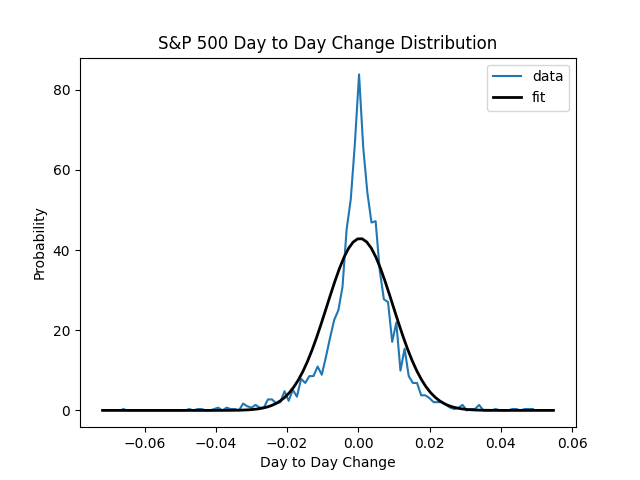
\includegraphics[width=0.8\textwidth]{../day_to_day_change.png}
    \caption{Histogram of the day to day changes of the S\&P 500 index over the timeframe of our dataset, and a fitted normal distribution.}
    \label{fig:histogram}
\end{figure}
To more quantifiablely demonstrate that the returns are not normally distributed, let us perform a Kolmogorov-Smirnov test at 
a significance level of $0.001$. The null hypothesis of the Kolmogorov-Smirnov test is that the distribution of the 
day to to day change in the price of the asset is normally distributed according to the fitted normal distribution. At this confidence level,
we can reject the null hypothesis of normallity for all but $6$ of the $428$ assets. 

% This is plotted in figure \ref{fig:ks_test}.\\\\

% To evaluate the assumption that the returns of the assets are normally distributed, let us introduce two measures, the skewness and the kurtosis 
% of a distribution. We define the skewness as
% \begin{equation}
%     \gamma = \frac{\mu_3}{\sigma^3}
% \end{equation}
% Where $\mu_3=\mathbb{E}[(X-\mu)^3]$ is the third central moment of the distribution, and $\sigma$ is the standard deviation of the distribution. We define the kurtosis as
% \begin{equation}
%     \kappa = \frac{\mu_4}{\sigma^4}
% \end{equation}
% Where $\mu_4=\mathbb{E}[(X-\mu)^4]$ is the fourth central moment of the distribution, and $\sigma$ is the standard deviation of the distribution. 
% An intuitive way to think about the skewness is that it measures the asymmetry of the distribution. If the distribution is symmetric, then the skewness is zero.
% Likewise an intuitive way to think about the kurtosis is that it measures the thickness of the tails of the distribution. If the distribution has the same tails as a normal distribution, then the kurtosis is $3$.
% Therefore we can define the excess kurtosis as $\kappa-3$. This 
% is an important measure that we need to account for when we are modeling the returns of the assets, since the tails of the distribution can cause large losses, that if 
% we use a normal distribution to model the returns, we will serverly underestimate the probability of.\\\\
% For a normal distribution we have that $\gamma=0$ and $\kappa=3$. Thus we have plotted in figure \ref{fig:skewness_kurtosis} the skewness and the excess kurtosis of the returns of the assets.
% of the assets with the highest and lowest $|\gamma|$ and $|\kappa-3|$.\\\\
% TODO: Add figure
\section{Method}
Our method consists of two parts. The first part is to model the returns of a set of assets with a nonparametric Kernel Density Estimation with 
a multivariate Gaussian Kernel. The second part is to isolate the assets into smaller subsets that are highly correlated with itself through 
spectral clustering.
\subsection{Kernel Density Estimation}
Effectively with Kernel Density Estimation what we try to do is with a kernel function, we 
smooth a normalized histogram of the data. The kernel function is a function that is centered around a point, and is symmetric around that point.
Mathematically, we can write the kernel density estimation for the the $pdf$ of a random variable $X$ as
\begin{equation}
\hat{f}_{\theta}(x) = \frac{1}{n} \sum_{i=1}^n K_{\theta}(x-x_i')
\end{equation}
where $K_{\theta}$ is the kernel function, and $\theta$ are the parameters of the Kernel, and $x_i'$ is the $i$th training point. 
In our case $x_i'$ is a $m$ dimensional vector representing the daily change for each of the $m$ stocks in our dataset.
We assume that that each kernel function is normalized $\int_{\mathbb{R}^d} K_{\theta}(x) dx = 1$
\subsubsection{Optimizing the Kernel Parameters}
We would want to find the optimal Kernel Parameters, we would want to minimize the log likelihood function, ie we would want to minimize:
\begin{equation}
    \mathcal{L}(x_1,\dots,x_k) = -\sum_{i=1}^k \log(\hat{f}_{\theta}(x_i))
\end{equation}
Where $x_1,\dots,x_k$ are the test points.\\\\
Now let us restrict our considerations to the case of a gaussian multivariate kernel. We have that
$$K_{\Sigma}(x) = \frac{1}{\sqrt{(2\pi)^d|\Sigma|}}\exp\left(-\frac{1}{2}x^T\Sigma^{-1}x\right)$$
Where $\Sigma$ is the covariance matrix for the kernel. Because the 
covariance matrix is symmetric positive semidefinite 
we can express $\Sigma$ as $\Sigma = R^TR$ through Cholesky decomposition.
We have that the derivative of the 
weighted log likelihood function is given by:
\begin{align*}
    \frac{\partial}{\partial R}\mathcal{L}(x_1,\dots,x_k) &= -\sum_{i=1}^k \frac{1}{\hat{f}_{\theta}(x_i)} \frac{\partial \hat{f}_{\theta}(x_i)}{\partial R}
\end{align*}
We have that 
\begin{align*}
    \frac{\partial |\Sigma|}{\partial R} &= \frac{\partial |R^TR|}{\partial R} \\
    &= 2|\Sigma|R^{-T}
\end{align*}
Therefore we have that 
\begin{equation}
    \frac{\partial}{\partial R}\frac{1}{\sqrt{(2\pi)^d|\Sigma|}} = -R^{-T}\frac{1}{\sqrt{(2\pi)^d|\Sigma|}}
\end{equation}
%     \frac{\partial}{\partial R}\frac{1}{\sqrt{(2\pi)^d|\Sigma|}} &= -R^{-T}\frac{1}{\sqrt{(2\pi)^d}}
% \end{align*}
We also have that:
\begin{equation}
    \frac{\partial}{\partial R} e^{\frac{1}{2}x^T\Sigma^{-1}x} = \frac{1}{2}e^{\frac{1}{2}x^T\Sigma^{-1}x} \frac{\partial}{\partial R} x^T(R^{-1}R^{-T})x
\end{equation}
$\frac{\partial}{\partial R} x^T(R^{-1}R^{-T})x$ is very difficult to calculate, so we must approximate it. First we note that for 
a function $f(\mathbf{x})$ that takes in a vector $\mathbf{x}$ we have that the first order taylor expansion is given by:
\begin{equation}
    f(\mathbf{x}+\Delta \mathbf{x}) \approx f(\mathbf{x}) + \frac{\partial f(\mathbf{x})}{\partial \mathbf{x}}\Delta \mathbf{x}
\end{equation}
Where $\frac{\partial f(\mathbf{x})}{\partial \mathbf{x}}$ is a $1\times d$ vector, if $\mathbf{x}$ is a $d$ dimensional vector. Therefore 
we argue that a generalization to a function of a matrix $\mathbf{X}$ is given by:
\begin{equation}
    f(\mathbf{X}+\Delta \mathbf{X}) \approx f(\mathbf{X}) + \mathbf{1}^T\left(\frac{\partial f(\mathbf{X})}{\partial \mathbf{X}}\circ \Delta \mathbf{X}\right)\mathbf{1}
\end{equation}
Where $\circ$ is the Hadamard product, and $\mathbf{1}$ is a $d\times 1$ vector of ones. We note that $\mathbf{1}^T\left(\frac{\partial f(\mathbf{X})}{\partial \mathbf{X}}\circ \Delta \mathbf{X}\right)\mathbf{1}$
equals to $\Tr\left(\left(\frac{\partial f(\mathbf{X})}{\partial \mathbf{X}}\right)^T\mathbf{X}\right)$. We have for our specific case:
\begin{align*}
    x^T((R+\delta R)^{-1}(R+\delta R)^{-T})x &\approx x^T(R^{-1}R^{-T})x + \Tr\left(\left(\frac{\partial(x^TR^{-1}R^{-T})x}{\partial R}\right)^T  \delta R\right)
\end{align*}
We note that for small pertubations, $(R+\delta R)^{-1} \approx R^{-1} - R^{-1}\delta R R^{-1}$, and therefore:
\begin{align*}
    x^T (R^{-1} - R^{-1}\delta R R^{-1})(R^{-T} - R^{-T}\delta R^T R^{-T})x &\approx x^T(R^{-1}R^{-T})x + \Tr\left(\left(\frac{\partial(x^TR^{-1}R^{-T})x}{\partial R}\right)^T  \delta R\right)
\end{align*}
Only keeping the zeroth order and first order terms, we have that:
\begin{align*}
    x^T(R^{-1}R^{-T})x - x^T \left(R^{-1}\delta R R^{-1}R^{-T} + R^{-1}R^{-T}\delta R^T R^{-T}\right)x \approx& x^T(R^{-1}R^{-T})x \\&+ \Tr\left(\left(\frac{\partial(x^TR^{-1}R^{-T})x}{\partial R}\right)^T  \delta R\right)\\
\end{align*}
\begin{equation}
    - x^T \left(R^{-1}\delta R R^{-1}R^{-T} + R^{-1}R^{-T}\delta R^T R^{-T}\right)x \approx \Tr\left(\left(\frac{\partial(x^TR^{-1}R^{-T})x}{\partial R}\right)^T  \delta R\right)\\
\end{equation}
Because the left side is a scalar, we can apply an trace operator to both sides, and noting that $R^{-1}R^{-T}=\Sigma^{-1}$, we have that:
\begin{align*}
    -\Tr\left(x^T \left(R^{-1}\delta R \Sigma^{-1} + \Sigma^{-1}\delta R^T R^{-T}\right)x\right) &\approx \Tr\left(\left(\frac{\partial(x^TR^{-1}R^{-T})x}{\partial R}\right)^T  \delta R\right)\\
    -\Tr\left(x^T R^{-1}\delta R \Sigma^{-1}x\right) -\Tr\left( x^T\Sigma^{-1}\delta R^T R^{-T}x\right)&\approx\\
    -\Tr\left(x^T R^{-1}\delta R \Sigma^{-1}x\right)-\Tr\left( x^TR^{-1}\delta R \Sigma^{-T} x\right)&\approx\\
    -2\Tr\left(x^T R^{-1}\delta R \Sigma^{-1}x\right) &\approx\\
    -2\Tr\left( \Sigma^{-1}xx^T R^{-1}\delta R\right) &\approx \Tr\left(\left(\frac{\partial(x^TR^{-1}R^{-T})x}{\partial R}\right)^T  \delta R\right)
\end{align*}
Therefore we can see that 
\begin{equation}
    \frac{\partial}{\partial R} x^T(R^{-1}R^{-T})x \approx -2\Sigma^{-1}xx^T R^{-1}
\end{equation}
Therefore we have that:
\begin{equation}
    \frac{\partial}{\partial R} e^{\frac{1}{2}x^T\Sigma^{-1}x} \approx -e^{\frac{1}{2}x^T\Sigma^{-1}x} \Sigma^{-1}xx^T R^{-1}
\end{equation}
Therefore we have that
\begin{equation}
    \frac{\partial}{\partial R} K_{\Sigma}(x) \approx -K_{\Sigma}(x)R^{-T} - K_{\Sigma}(x)\Sigma^{-1}xx^T R^{-1}
\end{equation}
And thus we have:
\begin{equation}
    \frac{\partial}{\partial R} \hat{f}(x) \approx -\sum_{i=1}^n K_{\theta}(x-x_i')\left(R^{-T} - \Sigma^{-1}(x-x_i')(x-x_i')^T R^{-1}\right)
\end{equation}
Therefore we have that:
\begin{equation}
    \frac{\partial}{\partial R}\mathcal{L}(x_1,\dots,x_k) \approx \sum_{i=1}^k \frac{1}{\hat{f}(x_i)} \sum_{j=1}^n K_{\theta}(x_i-x_j')\left(R^{-T} - \Sigma^{-1}(x_i-x_j')(x_i-x_j')^T R^{-1}\right)
\end{equation}
From this we can just optimize $R$ using stochastic gradient descent, or other more advanced methods such as ADAM. For this 
report we just used stochastic gradient descent with $\eta=0.01$ and $T=10$ epochs with minibatching the data into 20 batches.
\subsubsection{Obtaining a More Accurate Sharpe Ratio}
As we noted before what we want to optimize is the sharpe ratio:
What we want to optimize is the sharpe 
ratio, which is given by: 
\begin{equation}
    \frac{\mathbb{E}[R_p]}{\sigma_p}
\end{equation}
If we have that the weights for each of the $m$ stocks is given by a vector $w$, then we can write the expected return as:
\begin{equation}
    \mathbb{E}[R_p] = \mathbb{E}[w^T x]
\end{equation}
Where $x$ is the vector of daily returns for each of the $m$ stocks. We have that this is given by:
\begin{align}
    \mathbb{E}[w^T x] &= \int_{\mathbb{R}^{m}} w^T x \hat{f}_h(x) dx \\
    &= \frac{1}{n} \sum_{i=1}^k\int_{\mathbb{R}^{m}} w^T xK_{\Sigma}(x-x_i') dx
\end{align}
Now we can use the fact that the kernel function is symmetric to get:
\begin{align*}
    \int_{\mathbb{R}^{m}} xK_{\Sigma}(x-x_i') dx & = \int_{\mathbb{R}^{m}} (x_i'-u)K_{\Sigma}(u) du 
\end{align*}
Where $u=x-x_i'$, because $K_{\Sigma}(u)$ is symmetric (even) about $u=0$. we have that $\int_{\mathbb{R}^{m}}uK_{\Sigma}(u) du = 0$, thus we have that 
\begin{align}
    \int_{\mathbb{R}^{m}} xK_{\Sigma}(x-x_i') dx & = \int_{\mathbb{R}^{10}}x_i'K_{\Sigma}(u) du \\
    &= x_i'
\end{align}
Therefore we have that:
\begin{align}
    \mathbb{E}[w^T x] &= \frac{1}{n} \sum_{i=1}^nw^T x_i'
    \label{eq:expectedreturn}
\end{align}
Now we need to find the variance of the portfolio, which is given by:
\begin{align}
    \sigma_p^2 & = \mathbb{E}[(w^T x)^2] - \mathbb{E}[w^T x]^2
    \label{eq:variance}
\end{align}
From equation (\ref{eq:expectedreturn}) we have that, $\mathbb{E}[w^T x]^2=\left(\frac{1}{n} \sum_{i=1}^nw^T x_i'\right)^2$.
We have that $\mathbb{E}[(w^T x)^2]$ is given by:
\begin{align}
    \mathbb{E}[(w^T x)^2] &= \int_{\mathbb{R}^{m}} (w^T x)^2 \hat{f}_h(x) dx \\
    &= \frac{1}{n} \sum_{i=1}^n\int_{\mathbb{R}^{m}} (w^T x)^2 K_{\Sigma}(x-x_i') dx
\end{align}
We have that because $w^Tx$ is a scalar, we have that $(w^Tx)^T=x^Tw=w^Tx$, therefore we have that:
\begin{align}
    \mathbb{E}[(w^T x)^2] &= \frac{1}{n} \sum_{i=1}^n\int_{\mathbb{R}^{m}} w^Txx^Tw K_{\Sigma}(x-x_i') dx \\
    &= \frac{1}{n} \sum_{i=1}^nw^T\left(\int_{\mathbb{R}^{m}} xx^T K_{\Sigma}(x-x_i') dx\right)w\\
    &= w^T\left(\frac{1}{n}\sum_{i=1}^n\int_{\mathbb{R}^{m}} xx^T K_{\Sigma}(x-x_i') dx\right)w
    \label{eq:variance2}
\end{align}
For a gaussian kerenel with covariance matrix $\Sigma$, we have that:
\begin{equation}
    \int_{\mathbb{R}^{10}} xx^T K_{\Sigma}(x-x_i') dx = x_i'x_i'^T + \Sigma
\end{equation}
Therefore we have that 
equation (\ref{eq:variance2}) becomes
\begin{align}
    \mathbb{E}[(w^T x)^2]
    &= w^T\left(\frac{1}{n}\sum_{i=1}^nx_i'x_i'^T + \Sigma\right)w\\
    &=  w^T\left(\Sigma+\frac{1}{n}\sum_{i=1}^nx_i'x_i'^T\right)w\\
    &=  w^T\Sigma w + w^T\left(\frac{1}{n}\sum_{i=1}^nx_i'x_i'^T\right)w
\end{align}
Therefore we have that equation (\ref{eq:variance}) becomes:
\begin{equation}
    \sigma_p^2 =w^T\Sigma w + w^T\left(\frac{1}{n}\sum_{i=1}^nx_i'x_i'^T\right)w-\left(\frac{1}{n} \sum_{i=1}^nw^T x_i'\right)^2
\end{equation}
We have: $\left(\frac{1}{n} \sum_{i=1}^nw^T x_i'\right)=w^T\left(\frac{1}{n} \sum_{i=1}^nx_i'\right)=\left(\frac{1}{n} \sum_{i=1}^nx_i'\right)^Tw$, therefore we have that:
\begin{equation}
    \sigma_p^2 = w^T\left(\Sigma +  \frac{1}{n}\sum_{i=1}^nx_i'x_i'^T - \left(\frac{1}{n} \sum_{i=1}^nx_i'\right)\left(\frac{1}{n} \sum_{i=1}^nx_i'\right)^T\right)w
\end{equation}
Thus we can see that with Kernel Density Estimation we have effectively created a pseduo-covariance matrix
\begin{equation}
    \hat{\Sigma} = \Sigma +  \frac{1}{n}\sum_{i=1}^nx_i'x_i'^T -\left(\frac{1}{n} \sum_{i=1}^nx_i'\right)\left(\frac{1}{n} \sum_{i=1}^nx_i'\right)^T
\end{equation}
Therefore we can use this instead of the sample covariance matrix in the fractional programming problem to find the optimal
portfolio weights that maximize the Sharpe ratio.\\\\
\subsection{Spectral Clustering}
Our experimentation found that Kernel Density Estimation would fail on high dimensional datasets such as 
the 400+ stocks we used in our experiments. Therefore we decided to adopt a strategy of dimensionality reduction. We first 
performed Kernel Density Estimation on a subset of stocks that were from the same "sector," and then generating an optimal portfolio
of these stocks of the dataset. Then we applied Kernel Density Estimation to the dataset of optimal portfolios for 
each sector.\\\\
To identify the sectors we used spectral clustering on the correlation matrix, specifically we used the negative of the 
correlation matrix as the adjacency matrix, with the diagonal elements zeroed out. We chose to use this method because 
we wanted to identify clusters of stocks that were highly correlated with each other.\\\\
To determine the optimal number of clusters we used the eigengap heuristic as proposed by \cite{von2007tutorial} and 
\cite{ng2002spectral}. The eigengap is defined as the difference between the eigenvalue of the $k$th smallest
eigenvalue and the $(k+1)$th smallest eigenvalue. Then the optimal number of clusters is the value of $k$ that maximizes
the eigengap. Because our "graph" created by the covariance matrix is fully connected, we had to limit the number of 
clusters to a minimum of 5 and a maximum of 50. We found that the optimal number of clusters was 17.
\section{Results}
\subsection{Spectral Clustering}
As we discussed previously, we used the eigengap, we have plotted the eigenvalues and the eigengap for the 
for the sample covariance matrix measured from the train set in Figure \ref{fig:eigenvalues_and_eigengap}. We can see that the eigengap is maximized at 17.\\\\
\begin{figure}[t]
    \centering
    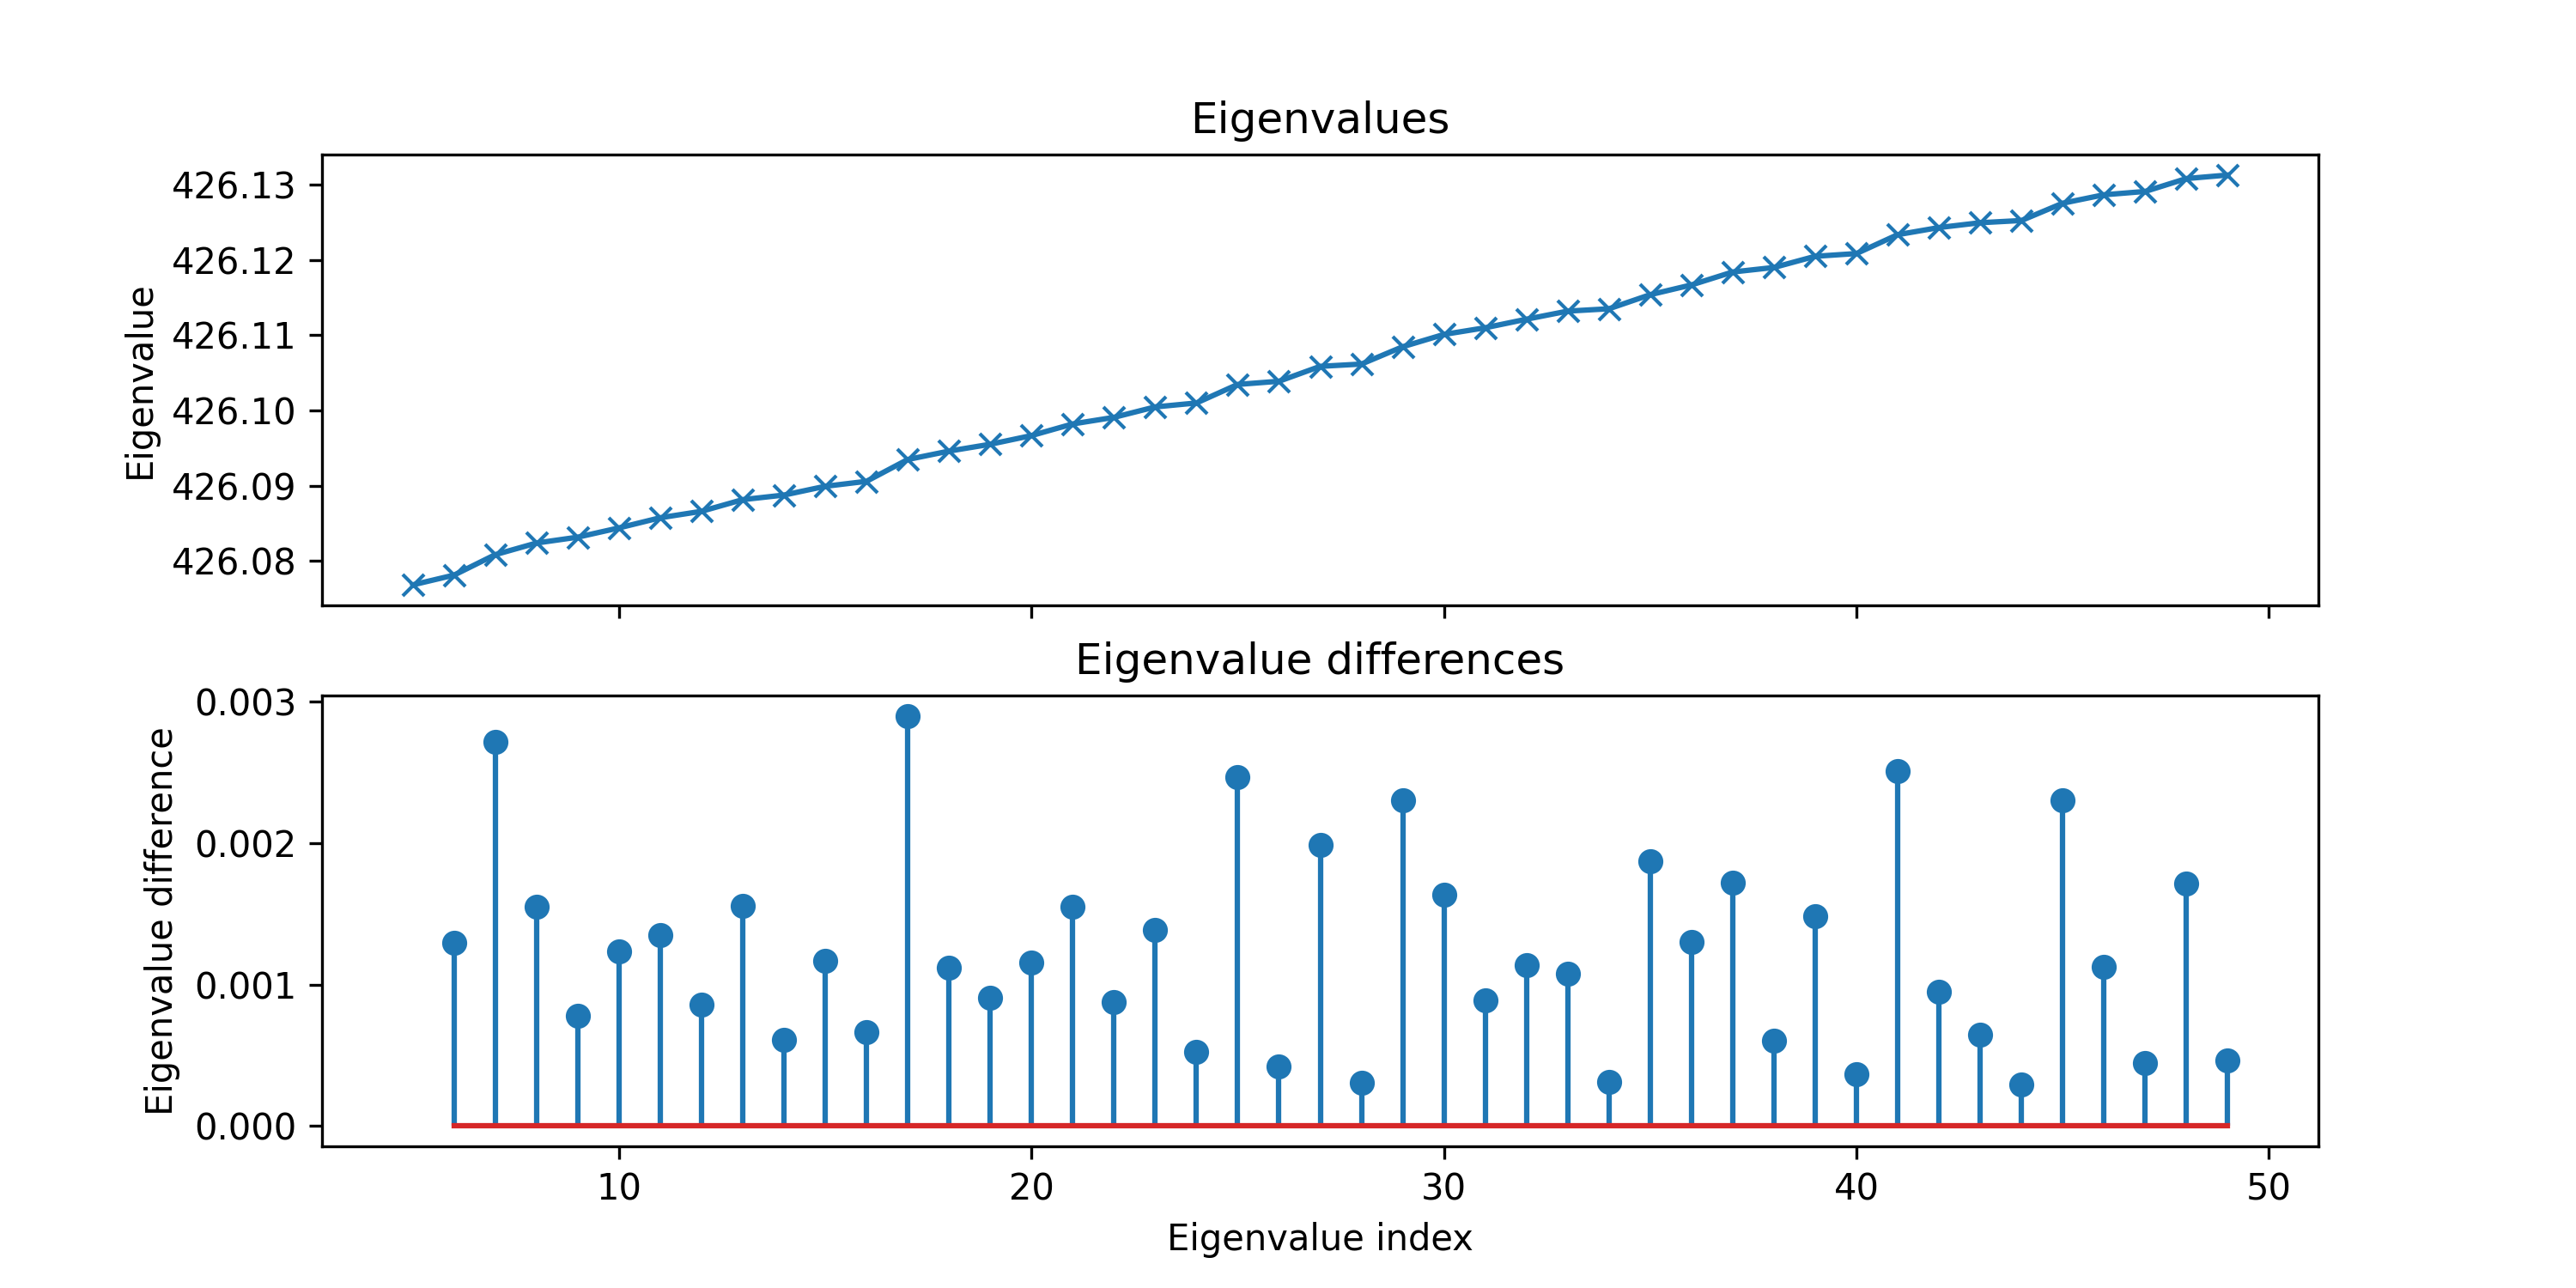
\includegraphics[width=0.9\textwidth]{../eigenvalues.png}
    \caption{Eigenvalues and Eigengap}
    \label{fig:eigenvalues_and_eigengap}
\end{figure}
We also have plotted out the sample correlation matrix, before clustering, and after clustering in Figure \ref{fig:correlation_matrix}. We can see that the correlation matrix after clustering has a block diagonal structure, which is what we would expect from a clustering algorithm.\\\\
\begin{figure}[t]
    \centering
    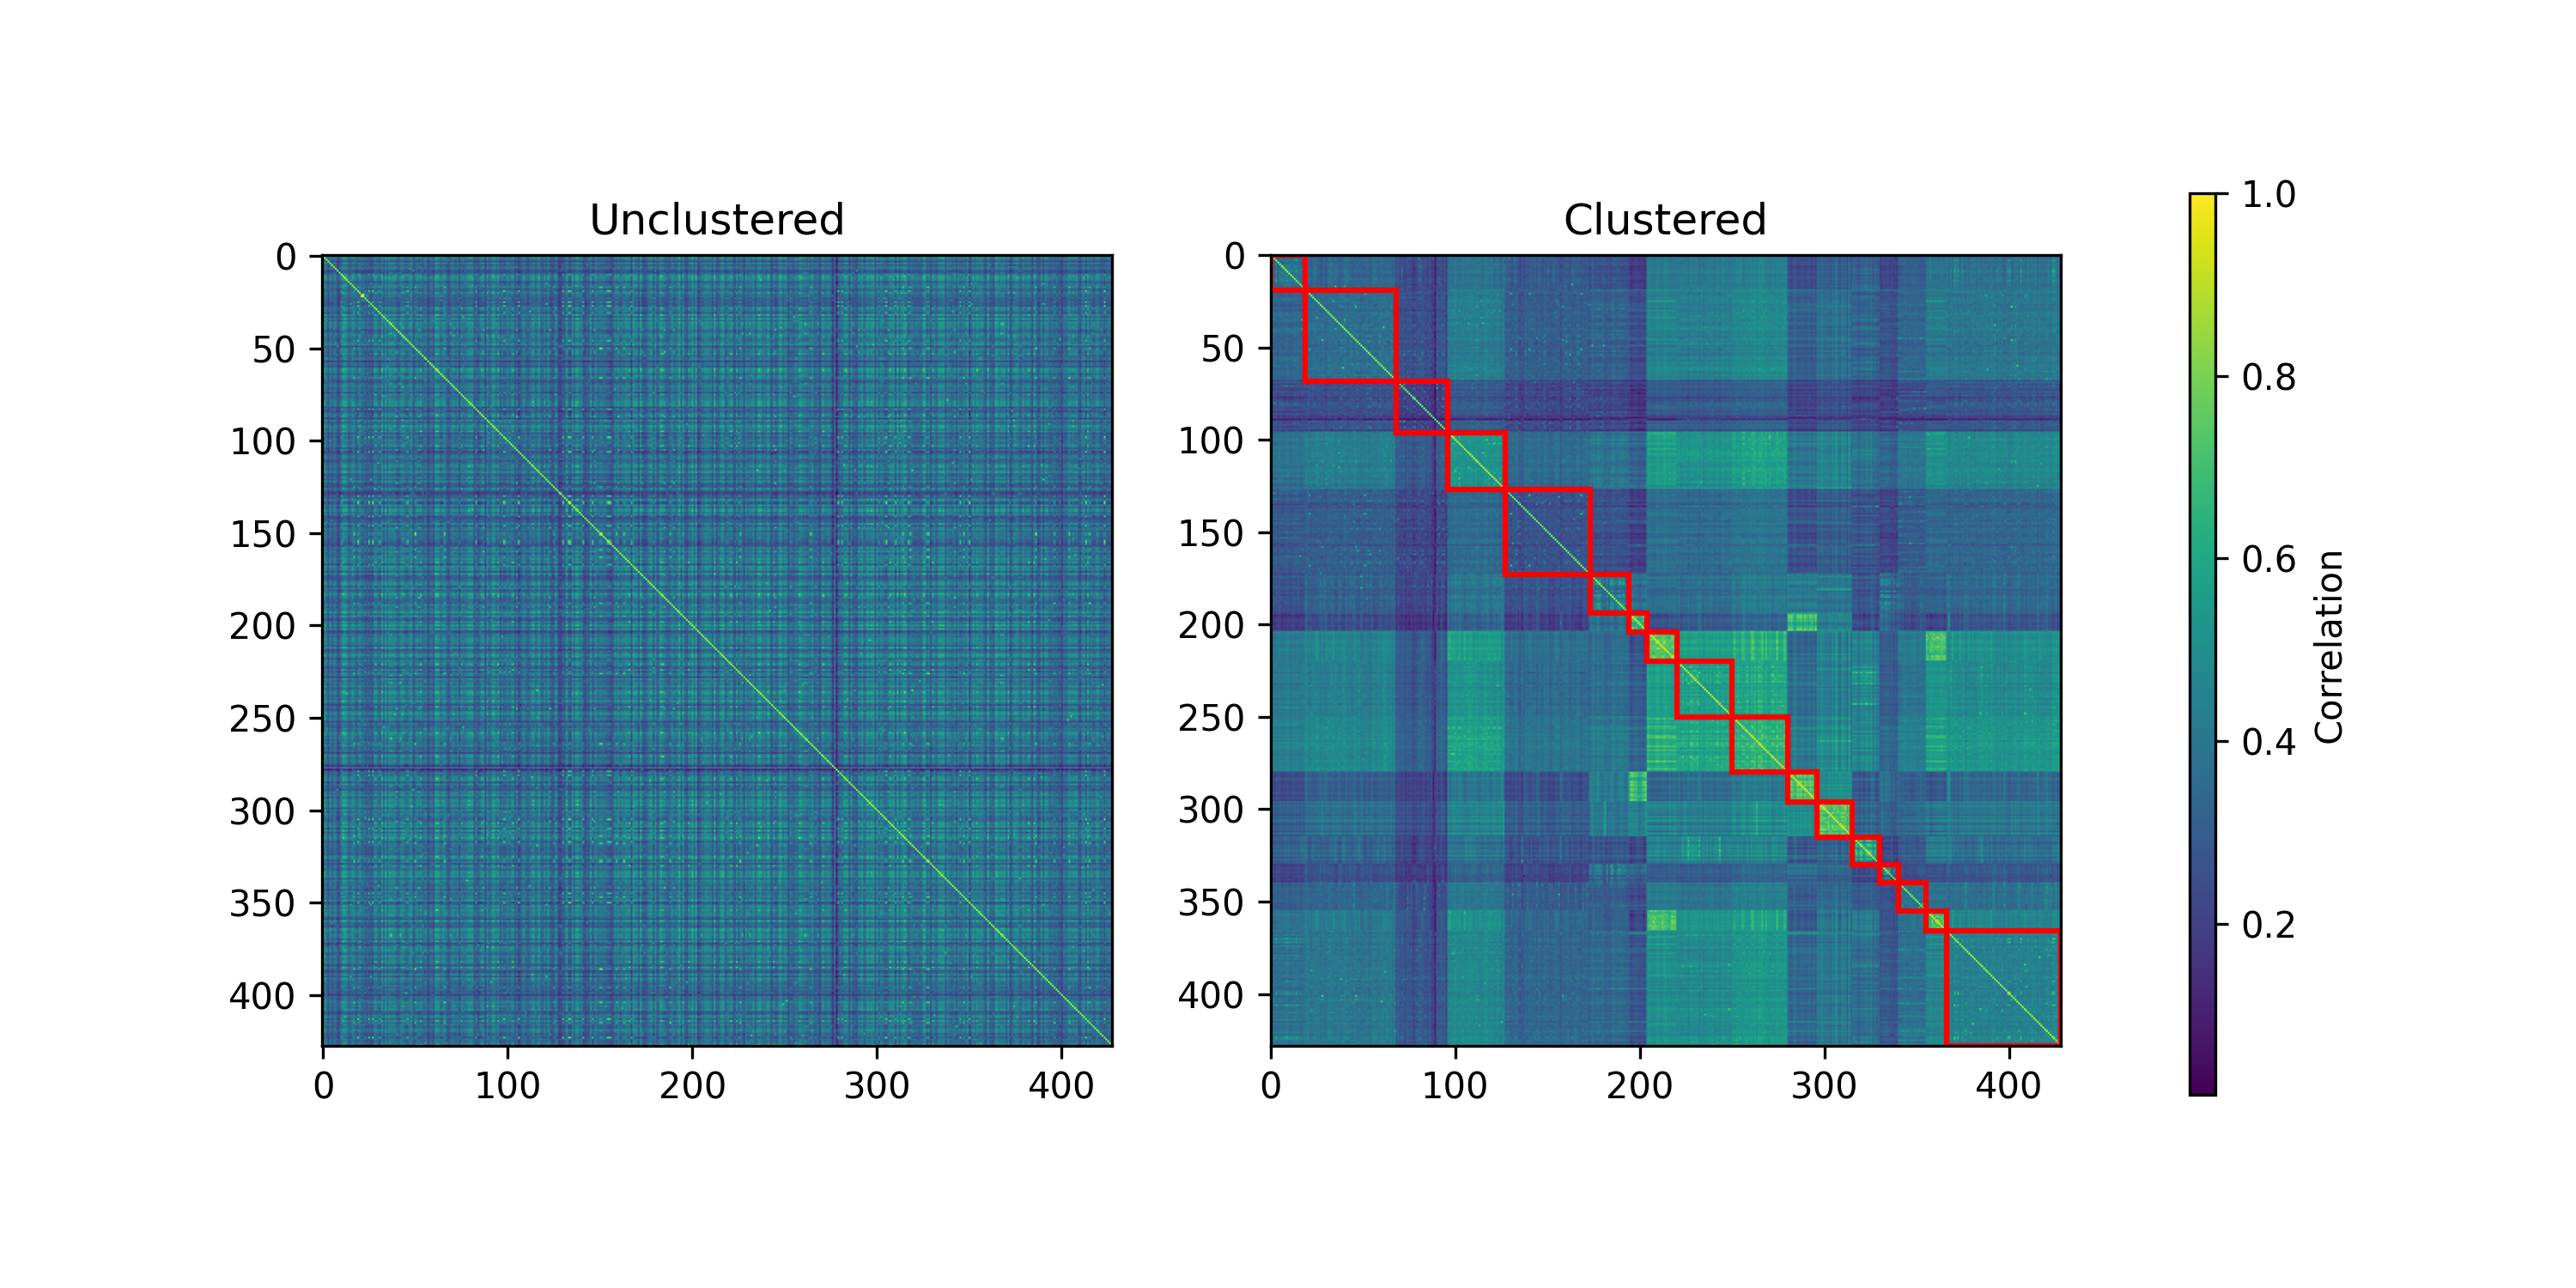
\includegraphics[width=0.9\textwidth]{../clustered_corr.png}
    \caption{Correlation Matrix Before and After Clustering, with the Clustered blocks highlighted in red}
    \label{fig:correlation_matrix}
\end{figure}
To investigate how the stocks are clusters, we report the stock ticker, and corresponding company name for a select 
number of clusters in Table \ref{tab:clusters7} and Table \ref{tab:clusters10}. We can see that the clustering algorithm was able to identify clusters,
with the stocks in cluster 7 being mostly financial companies, and the stocks in cluster 10 being mostly energy companies.\\\\

\begin{table}
    \centering
    \begin{tabular}{|c|c|}
        \hline 
        Ticker & Company \\
        \hline
        AMP & Ameriprise Financial, Inc. \\
        BK & The Bank of New York Mellon Corporation \\
        C & Citigroup Inc. \\
        FITB & Fifth Third Bancorp \\
        JPM & JPMorgan Chase \& Co. \\
        LNC & Lincoln National Corporation \\
        MET & MetLife, Inc. \\
        NTRS & Northern Trust Corporation \\
        PNC & The PNC Financial Services Group, Inc. \\
        PRU & Prudential Financial, Inc. \\
        RJF & Raymond James Financial, Inc. \\
        STT & State Street Corporation \\
        HIG & The Hartford Financial Services Group, Inc. \\
        TFC & Truist Financial Corporation \\
        USB & U.S. Bancorp \\
        WFC & Wells Fargo \& Company \\
        \hline
    \end{tabular}
    \caption{The tickers in cluster 7}
    \label{tab:clusters7}
\end{table}

\begin{table}
    \centering
    \begin{tabular}{|c|c|}
        \hline 
        Ticker & Company \\
        \hline
        LNT & Alliant Energy Corporation \\
        AEE & Ameren Corporation \\
        AEP & American Electric Power Company, Inc. \\
        ATO & Atmos Energy Corporation \\
        CNP & CenterPoint Energy, Inc. \\
        CMS & CMS Energy Corporation \\
        D & Dominion Energy, Inc. \\
        DTE & DTE Energy Company \\
        EVRG & Evergy, Inc. \\
        ES & Eversource Energy \\
        NEE & NextEra Energy, Inc. \\
        NI & NiSource Inc. \\
        PNW & Pinnacle West Capital Corporation \\
        PEG & Public Service Enterprise Group Incorporated \\
        SRE & Sempra \\
        XEL & Xcel Energy Inc. \\
        \hline
    \end{tabular}
    \caption{The tickers in cluster 10}
    \label{tab:clusters10}
\end{table}
\subsection{Kernel Density Estimation}
We investigated 3 methods of portfolio optimization, the first was the standard Markowitz portfolio optimization, 
the second was applying Kernel Density Estimation straight to the dataset, and the third was applying Kernel Density
Estimation to each sector, and then applying Kernel Density Estimation to the dataset of optimal portfolios. In our 
table we denote this method as "Spectral Clustering + KDE."\\\\
The sharpe ratio each portfolio was able to achive is shown in Table \ref{tab:sharpe_ratios}. We can see that the
our method of Spectral Clustering + KDE was able to achieve the highest sharpe ratio. We also reported out the 
average year over year (YoY) returns for each method in Table \ref{tab:YoY_returns}.
\begin{table}[H]
    \centering
    \begin{tabular}{|c|c|c|}
        \hline
        Method & Sharpe Ratio (train) & Sharpe Ratio (test)\\
        \hline
        S\&P 500 & 0.804 & 0.709 \\
        Markowitz & 2.266 & 1.199 \\
        KDE & 1.201 & 0.920 \\
        Spectral Clustering + KDE & 1.969 & 1.424\\
        \hline
    \end{tabular}
    \caption{Sharpe Ratios for each method}
    \label{tab:sharpe_ratios}
\end{table}
\begin{table}[H]
    \centering
    \begin{tabular}{|c|c|c|}
        \hline
        Method & YOY (train) & YOY (test)\\
        \hline
        S\&P 500 & 11.352 \% & 9.947\% \\
        Markowitz & 37.699\% & 15.969\% \\
        KDE & 19.362\% & 12.743\% \\
        Spectral Clustering + KDE & 25.246\% & 17.398\%\\
        \hline
    \end{tabular}
    \caption{Sharpe Ratios for each method}
    \label{tab:YoY_returns}
\end{table}
As we can see the Spectral Clustering + KDE method was able to achieve the highest sharpe ratio,
and the highest YoY returns on the test set. And was able to outperform the S\&P 500 by 7.451\% in terms of YoY returns
in the test set.
\section{Discussion}
While we were able to achieve a higher sharpe ratio and YoY returns on the test set, we believe that there is additional 
performance that can be tuned out of our model. When we trained it, we noticed "ping-ponging" behavior, where the 
negative log likelihood would increase and decrease. Likewise we noticed that optimization algorithm was highly 
sensitive to the learning rate and initial conditions. We believe that this is due to the fact that we used a fairly 
simple optimization algorithm, and further work can be done with more sophisticated optimization algorithms such as stochastic
gradient descent with momentum and a cosine annealing learning rate scheduler, or using Adam \cite{kingma2014adam}.\\\\
We also noticed that the algorithm would often produce a $\Sigma$ that was not positive semidefinite or that was 
poorly numerically conditioned, leading to the production of NaN values by the kernel density estimation algorithm, which would 
cause the optimization algorithm to fail. Thus one direction of future work would be to make the algorithm more numerically stable.
Another further direction would be to investigate other kernels that can have "fatter" tails than the Gaussian kernel,
such as a multivariate t-distribution kernels.\\\\
Other directions also include developing a model that can handle non stationary distributions, the other drawback of 
MPT that we discussed in the introduction.
%include references
\bibliographystyle{plain}
\bibliography{references}
\end{document}

